\chapter{Galois表示之二：模曲线、模形式与Hecke代数}\label{L8}
\lecturedate{2020/03/11}\sourcepage{61}
本讲概述\lref{L7}所介绍的Eichler--Shimura、Deligne定理的证明。
\section{模曲线与模形式}\label{L8S1}\idx{模曲线}
根据上一讲关于椭圆曲线的讨论，若要参数化所有复椭圆曲线在$\C$上的同构类，可以使用$j$不变量，或格$\Lambda$的位似类。可以假定$\Lambda=\Z\oplus\omega\Z$，其中$\omega\in\mathcal H$，$\mathcal H$是\lref{L6}中的上半平面。容易验证以下结论。
\originalnumber{1}
\begin{lemma}\label{L8S1O1}
设$\Lambda=\Z\oplus\omega\Z$，$\Lambda'=\Z\oplus\omega'\Z$。则$\Lambda$与$\Lambda'$位似，当且仅当存在$g=\begin{pmatrix}a&b\\c&d\end{pmatrix}\in\SL_2(\Z)$，使
\[\omega=g(\omega')=\frac{a\omega'+b}{c\omega'+d}.\]
\end{lemma}
因此，得到如下交换图：
\begin{figure}[H]\centering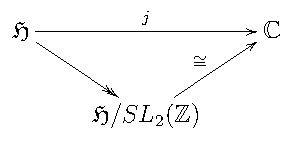
\includegraphics[width=0.2351\paperwidth]{images/L8-p061-j.pdf}\end{figure}
对任意有限指数子群$\Gamma\subset\SL_2(\Z)$，令$Y_\Gamma:=\mathcal H/\Gamma$，它是一维复解析流形。记$X_\Gamma$为$Y_\Gamma$的紧化\znote{「紧化」指把非紧的$Y_\Gamma$补成一个紧的对象。这里只需补上有限多个尖点，得到紧Riemann面，它同时是$\Q$上的光滑射影曲线。对一般的复流形，紧化并不唯一、往往要作额外选择；但在曲线情形，光滑紧化由$Y_\Gamma$唯一决定，所以「紧化」在这里没有歧义。[来源：nLab "compactification"，\url{https://ncatlab.org/nlab/show/compactification}（Last revised 2025-08-19；2026-11-14 访问）。]}，
\sourcepage{62}
则有
\begin{figure}[H]\centering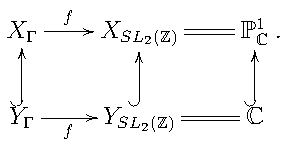
\includegraphics[width=0.2303\paperwidth]{images/L8-p062-compactification.pdf}\end{figure}
$X_\Gamma$是一条光滑射影曲线，并且$X_\Gamma\cong(\mathcal H\cup\mathbb P^1(\Q))/\Gamma$。由Riemann--Hurwitz公式，有
\begin{equation}\tag{1.1}\label{L8eq11}
2-2g(X_\Gamma)=2\deg f-\sum_P(e_P-1),
\end{equation}
其中$g(X_\Gamma)$为$X_\Gamma$的算术亏格，求和遍历$f$的所有分歧点$P\in X_\Gamma$，$e_P$为相应分歧指数。

本讲主要考虑下列两类同余子群：
\begin{align*}
\Gamma_1(N)&:=\left\{\begin{pmatrix}a&b\\c&d\end{pmatrix}\in\SL_2(\Z)\ \middle|\ a\equiv1,\ c\equiv0\pmod N\right\}\\
&\subset\Gamma_0(N):=\left\{\begin{pmatrix}a&b\\c&d\end{pmatrix}\in\SL_2(\Z)\ \middle|\ c\equiv0\pmod N\right\}.
\end{align*}
此前已经见过Hecke同余子群$\Gamma_0(N)$。映射$\begin{pmatrix}a&b\\c&d\end{pmatrix}\mapsto d\bmod N$将商$\Gamma_0(N)/\Gamma_1(N)$与$(\Z/N\Z)^\times$等同。它们的指数分别为
\[[\SL_2(\Z):\Gamma_0(N)]=N\prod_{p\mid N}(1+p^{-1}),\qquad [\SL_2(\Z):\Gamma_1(N)]=N^2\prod_{p\mid N}(1-p^{-2}).\]
对$j=0,1$，定义$Y_j(N):=Y_{\Gamma_j(N)}$，$X_j(N):=X_{\Gamma_j(N)}$。模曲线\znote{「模曲线」中的「模」指 moduli，即参数空间：这类曲线本来是用来参数化带附加结构的椭圆曲线的，而不是先有曲线再去找参数。作为复解析空间它是$\mathcal H/\Gamma$，作为代数对象它是$\Q$上的一维概形，两种描述的一致性由GAGA给出。模形式则是模曲线上的微分形式，二者是同源词。[来源：nLab "modular curve"，\url{https://ncatlab.org/nlab/show/modular+curve}（Last revised 2015-07-21；2026-11-14 访问）。]}$Y_1(N)$有如下解释：
\[Y_1(N)\ \xleftrightarrow{\;1\text{--}1\;}\ \left\{\begin{array}{l}\text{二元组$(E,P)$的同构类，其中$E$为$\C$上的椭圆曲线，}\\\text{$P\in E(\C)$为阶恰等于$N$的点。}\end{array}\right\}.
\]
\sourcepage{63}
这一双射由下列映射诱导：
\begin{equation}\tag{1.2}\label{L8eq12}
g_1:\tau\longmapsto\left(E=\C/(\Z\oplus\tau\Z),\quad P\equiv\frac1N\pmod{\Z\oplus\tau\Z}\right).
\end{equation}
\begin{exercise*}\label{L8S1EX1}
验证\eqref{L8eq12}中的$g_1$在$\Gamma_1(N)$作用下不变。

需注意：对于$\gamma=\begin{pmatrix}a&b\\c&d\end{pmatrix}\in\Gamma_1(N)$，有$\gamma(\tau)=(a\tau+b)/(c\tau+d)$，并且
\[(a\tau+b)\Z\oplus(c\tau+d)\Z=\Z\oplus\tau\Z\]
与$\Z\oplus\gamma(\tau)\Z$位似。因此，还要证明在乘以$c\tau+d$所给出的同构下，标记点满足
\[\frac1{N\gamma(\tau)}(a\tau+b)=\frac{c\tau+d}{N}\equiv\frac1N\pmod{\Z\oplus\tau\Z}.\]
\end{exercise*}
同样，有
\[Y_0(N)\ \xleftrightarrow{\;1\text{--}1\;}\ \left\{\begin{array}{l}\text{二元组$(E,G)$的同构类，其中$E$为$\C$上的椭圆曲线，}\\\text{$G\subset E(\C)$为阶$N$的循环子群。}\end{array}\right\}.\]
现在尝试在这些模曲线上构造通用族：
\begin{figure}[H]\centering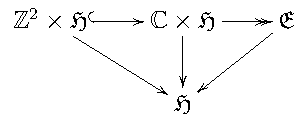
\includegraphics[width=0.2458\paperwidth]{images/L8-p063-family.pdf}\end{figure}
设$z$、$\tau$分别为$\C$、$\mathcal H$上的复坐标。群$\SL_2(\Z)$通过
\[\gamma\cdot(z,\tau)=\left(\frac z{c\tau+d},\gamma(\tau)\right),\qquad\gamma=\begin{pmatrix}a&b\\c&d\end{pmatrix},\]
作用于族$\mathcal E$。存在自然的零截面$0:\mathcal H\to\mathcal E$，它在每条看作加法群的曲线上选取零元。定义$\omega:=0^*\Omega^1_{\mathcal E/\mathcal H}$，则$\omega$由$dz$生成。对$\gamma\in\SL_2(\Z)$，有
\[\gamma^*dz=\frac1{c\tau+d}dz,\qquad \gamma^*\bigl(f(dz)^{\otimes k}\bigr)=(\gamma\cdot f)(c\tau+d)^{-k}(dz)^{\otimes k}.\]
因此，若$\Gamma$是$\SL_2(\Z)$的任意同余子群，$f\in M_k(\Gamma)$，则$f(dz)^{\otimes k}$是$\Gamma$不变的。可以把$M_k(\Gamma)$看成$H^0(\mathcal H,\omega^{\otimes k})$中在所有尖点处正则的$\Gamma$不变截面组成的子空间。此外，若
\sourcepage{64}
$\Gamma$在$\mathcal H$上的作用足够好，例如为自由作用，则$\omega$下降为$Y_\Gamma$上的线丛$\omega_Y$。若$\Gamma$进一步在尖点处正则作用，即
\[\Gamma_\infty\subset\left\{\begin{pmatrix}1&*\\0&1\end{pmatrix}\right\},\qquad \gamma\Gamma_c\gamma^{-1}\subset\left\{\begin{pmatrix}1&*\\0&1\end{pmatrix}\right\}\quad(\gamma c=\infty),\]
则要求$\omega_Y$的生成截面在尖点处的阶为0，便可以将它延拓到$X_\Gamma$。略微混用记号，将$\mathcal H$、$Y_\Gamma$和$X_\Gamma$上的这个线丛都记为$\omega$。有
\[M_k(\Gamma)=H^0(X_\Gamma,\omega^{\otimes k}).\]
另一方面，由形变理论，Kodaira--Spencer映射给出同构$R^1\pi_*T_{\mathcal E/\mathcal H}\cong T_{\mathcal H}$，其中$\pi:\mathcal E\to\mathcal H$为投影，$T_{\mathcal E/\mathcal H}$为$\pi$的相对切丛，$T_{\mathcal H}$为$\mathcal H$上的切丛。由凝聚对偶性——Serre对偶性的推广——得到
\begin{equation}\tag{1.3}\label{L8eq13}
\begin{aligned}
\Omega^1_{\mathcal H}&\cong(R^1\pi_*T_{\mathcal E/\mathcal H})^\vee
\cong\pi_*(\Omega^1_{\mathcal E/\mathcal H}\otimes T_{\mathcal E/\mathcal H}^\vee)\\
&\cong\pi_*((\Omega^1_{\mathcal E/\mathcal H})^{\otimes2})
\cong(0^*\Omega^1_{\mathcal E/\mathcal H})^{\otimes2}=\omega^{\otimes2}.
\end{aligned}
\end{equation}
\begin{exercise*}\label{L8S1EX2}
证明$\pi_*((\Omega^1_{\mathcal E/\mathcal H})^{\otimes2})\cong0^*((\Omega^1_{\mathcal E/\mathcal H})^{\otimes2})$。

提示：注意，$0(\mathcal H)$是$\mathcal E$中的一个除子。使用正合列
\[0\to\OO_{\mathcal E}(-0(\mathcal H))\to\OO_{\mathcal E}\to\OO_{0(\mathcal H)}\to0,\]
并证明$\pi_*((\Omega^1_{\mathcal E/\mathcal H})^{\otimes2}(-0(\mathcal H)))=0$，且$R^1\pi_*((\Omega^1_{\mathcal E/\mathcal H})^{\otimes2}(-0(\mathcal H)))$局部自由。
\end{exercise*}
由\eqref{L8eq13}，$\omega^{\otimes2}\cong\Omega^1_{Y_\Gamma}$，于是$(dz)^{\otimes2}$对应于$d\tau$。
% [Tutor Note: 原书 p64 作 "By (1.3), we have $\omega\cong\Omega^1_{Y_\Gamma}$"，与 \eqref{L8eq13} 的量纲不符，应为 $\omega^{\otimes2}\cong\Omega^1_{Y_\Gamma}$，译文按正确写法处理。]
\originalnumber{2}
\begin{note}[L8S1O2]
对任意$\gamma=\begin{pmatrix}a&b\\c&d\end{pmatrix}$，也可以直接看出
\[\gamma^*(dz)^{\otimes2}=\frac{(dz)^{\otimes2}}{(c\tau+d)^2},\qquad \gamma^*(d\tau)=\frac{d\tau}{(c\tau+d)^2},\]
这与$(dz)^{\otimes2}$对应于$d\tau$相容。
\end{note}
将$\omega$延拓到$X_\Gamma$时，在尖点处取局部参数$q$，有$d\tau$为$dq/q$的非零常数倍。因此，当$f\in S_2(\Gamma)$时，$f(dz)^{\otimes2}$给出$\Omega^1_{X_\Gamma}$的截面。一般地，得到
\[S_k(\Gamma)=H^0(X_\Gamma,\omega^{\otimes(k-2)}\otimes\Omega^1_{X_\Gamma}).\]
\sourcepage{65}
当$N\geq5$时，$\Gamma_1(N)$在$\mathcal H$上自由作用，且在尖点处正则；而$\Gamma_0(N)$的作用从来不是自由的，也不满足上述尖点正则条件。为从尖点模形式构造Galois表示，下面使用$X_1(N)$，并从现在起假定$N\geq5$。对$N\leq4$，也仍可以通过相应的模函子\znote{「模空间」是参数空间的正式说法：它的点与所参数化对象（这里是带水平结构的椭圆曲线）的同构类一一对应。严格的定义要用「模函子」，即把每个概形$S$映到「$S$上这类对象族」的集合。当对象带有非平凡自同构时，细模空间往往不存在，只能用粗模空间或模函子来代替；上一句提到的$N\leq4$正是这种情况。[来源：nLab "moduli space"，\url{https://ncatlab.org/nlab/show/moduli+space}（Last revised 2025-10-21；2026-11-14 访问）。]}完成整个构造，而不是直接使用这些模曲线。
\begin{exercise*}\label{L8S1EX3}
证明：$\Gamma_1(N)$在$\mathcal H$上自由作用，当且仅当$N\geq4$。

提示：先证明：对$\SL_2(\R)$中的非标量矩阵$\begin{pmatrix}a&b\\c&d\end{pmatrix}$，存在$\tau\in\mathcal H$满足$(a\tau+b)/(c\tau+d)=\tau$，当且仅当$(a+d)^2<4$。
\end{exercise*}
通用族$\mathcal E$也诱导$Y_1(N)$上的通用族$\mathcal E_Y$。它的半阿贝尔延拓的单位连通分支给出$X_1(N)$上的光滑群概形$\mathcal E_X$；尖点处的纤维同构于$\C^\times$。其原因是，当$\tau$趋向尖点$\infty$时，格$\Z\oplus\tau\Z$退化为秩1的格，因而尖点处的纤维为$\C/\Z\cong\C^\times$。
\section{Hecke算子与Hecke代数}\label{L8S2}\idx{Hecke算子}\idx{菱形算子}
由于$\Gamma_1(N)$是$\Gamma_0(N)$的正规子群，$\Gamma_0(N)$自然通过
\[f\longmapsto\gamma_k^*f(\tau):=(c\tau+d)^{-k}f(\gamma(\tau)),\qquad \gamma=\begin{pmatrix}a&b\\c&d\end{pmatrix}\in\Gamma_0(N),\]
作用于$S_k(\Gamma_1(N))$。$\Gamma_1(N)$在这一空间上的作用平凡，因此该作用下降为$\Gamma_0(N)/\Gamma_1(N)\cong(\Z/N\Z)^\times$的作用。对于$d\in(\Z/N\Z)^\times$，将其作用记为$\langle d\rangle$，称为\textbf{菱形算子}。也就是说，对任意右下角模$N$等于$d$的$\gamma\in\Gamma_0(N)$，都有$\langle d\rangle f=\gamma_k^*f$。由于$(\Z/N\Z)^\times$为交换群，有按特征标的分解
\[S_k(\Gamma_1(N))=\bigoplus_{\chi:(\Z/N\Z)^\times\to\C^\times}S_k(N,\chi),\]
其中$S_k(N,\chi)$与\lref{L6}的定义相同。此外，$S_k(N)=S_k(N,1)=S_k(\Gamma_1(N))^{\Gamma_0(N)}$。

Hecke代数\znote{Hecke代数可以理解为「所有Hecke算子一起生成的代数」：它作用在$S_k(\Gamma_1(N))$上，使后者成为它的模，而同时对角化就得到特征形式。在双陪集的语言里，它由$\Gamma\backslash\Delta/\Gamma$生成，乘法由双陪集的分解决定；对$\Gamma_1(N)$这个代数交换，这正是Hecke理论能继续做下去的关键。[来源：F. Diamond and J. Shurman, \textit{A First course in Modular forms}, Springer GTM 228 (2005), Section 7.9（本讲参考文献）。]}
\[\mathcal H_k(\Gamma_1(N)):=\Q[T_n\ (n\geq1),\ \langle d\rangle\ (d\in(\Z/N\Z)^\times)]\subset\End(S_k(\Gamma_1(N)))\]
是有限维交换$\Q$代数，其中$T_n$为Hecke算子。
\sourcepage{66}
这些算子形式地满足关系
\begin{equation}\tag{2.1}\label{L8eq21}
\sum_{n=1}^\infty T_n n^{-s}=\prod_{p\nmid N}(1-T_pp^{-s}+\langle p\rangle p^{k-1-2s})^{-1}\prod_{p\mid N}(1-T_pp^{-s})^{-1}.
\end{equation}
% [Tutor Note: 原书 p66 式 (2.1) 的第一个乘积下标也印作 $p\mid N$，与第二个相同；第一个应为 $p\nmid N$（否则不再是标准的 Euler 乘积，也与注 2.4 中 $L_f(s)$ 的展开不符）。原书 p68 的 $L_f(s)$ 展开同样如此。译文按 $p\nmid N$ 处理。]
下面定义$T_n$。对整数$N\geq4$、$n\geq1$，存在$Y_1(N)$上的有限平坦概形$T_1(N,n)$，其点可解释为如下三元组的同构类：
\[\left\{\begin{array}{l}(E,P,G),\quad\text{其中$E$为椭圆曲线，$P$为$E$上阶$N$的点，}\\\text{$G\subset E$为阶$n$的有限子群，且$G\cap\langle P\rangle=0$。}\end{array}\right\}.\]
自然的遗忘态射$s_Y:T_1(N,n)\to Y_1(N)$由$s_Y(E,P,G)=(E,P)$给出。另一个态射$t_Y:T_1(N,n)\to Y_1(N)$定义为$t_Y(E,P,G)=(E/G,\overline P)$。由于$\langle P\rangle\cap G=0$，$P$在$E/G$中的像$\overline P$仍然具有阶$N$。$s_Y,t_Y$都唯一延拓为完备正规曲线之间的有限平坦态射$s,t:\overline T_1(N,n)\to X_1(N)$：
\begin{figure}[H]\centering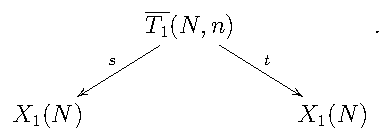
\includegraphics[width=0.3131\paperwidth]{images/L8-p066-correspondence.pdf}\end{figure}
于是有拉回及迹映射
\begin{align*}
t^*:S_k(\Gamma_1(N))&=H^0(X_1(N),\omega^{\otimes(k-2)}\otimes\Omega^1)\\
&\longrightarrow H^0(\overline T_1(N,n),t^*\omega^{\otimes(k-2)}\otimes\Omega^1),\\
s_*:H^0(\overline T_1(N,n),s^*\omega^{\otimes(k-2)}\otimes\Omega^1)&\longrightarrow H^0(X_1(N),\omega^{\otimes(k-2)}\otimes\Omega^1)\\
&=S_k(\Gamma_1(N)).
\end{align*}
由于$s,t$都是有限平坦映射，有$s_*\Omega^1\cong t_*\Omega^1\cong\Omega^1$。这里略微混用记号，$\Omega^1$始终表示相应曲线的余切丛；通过有限映射的微分拉回和迹映射定义上述箭头。存在通用同源$\nu:\mathcal E_T\twoheadrightarrow\mathcal E'_T$，其在$x=(E,P,G)\in T_1(N,n)$处的纤维为$E\twoheadrightarrow E/G$。有下列交换图；基底上的箭头为恒等映射：
\begin{figure}[H]\centering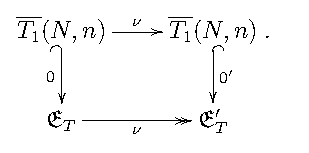
\includegraphics[width=0.2495\paperwidth]{images/L8-p066-isogeny.pdf}\end{figure}
\sourcepage{67}
由线丛$\omega$的函子性，在$T_1(N,n)$上有$t^*\omega\cong0'^*\Omega^1_{\mathcal E'_T/T}$及$s^*\omega\cong0^*\Omega^1_{\mathcal E_T/T}$。在特征0中，有限平坦的同源$\nu$在相对微分上诱导同构$\nu^*\Omega^1_{\mathcal E'_T/T}\cong\Omega^1_{\mathcal E_T/T}$，因而$\nu^*t^*\omega\cong s^*\omega$。有自然映射
\begin{figure}[H]\centering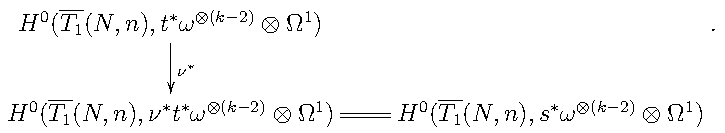
\includegraphics[width=0.5842\paperwidth]{images/L8-p067-pullback.pdf}\end{figure}
定义Hecke算子$T_n=s_*\circ\nu^*\circ t^*$\znote{这里用对应（correspondence）定义$T_n$，经典的说法则是双陪集：$T_n$对应双陪集$\Gamma\begin{pmatrix}1&0\\0&n\end{pmatrix}\Gamma$，把它分解为$\bigsqcup_i\Gamma\alpha_i$后，作用就是$f\mapsto\sum_i f|_k\alpha_i$。两种说法等价：对应的两个投影$s,t$正是双陪集各分支的「来源」与「去向」。用对应来写的好处是它对任意概形都说得通。[来源：nLab "double coset"，\url{https://ncatlab.org/nlab/show/double+coset}（Last revised 2019-08-01；2026-11-14 访问）。]}，使下图交换：
\begin{figure}[H]\centering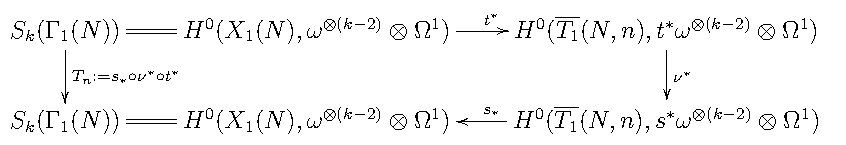
\includegraphics[width=0.6818\paperwidth]{images/L8-p067-Hecke.pdf}\end{figure}
\originalnumber{1}
\begin{note}[L8S2O1]
当$n=p$为素数时，Hecke算子$T_p$可以显式定义为：对任意$f\in S_k(\Gamma_1(N))$，
\[T_pf(\tau)=\frac1p\sum_{j=0}^{p-1}f\left(\frac{\tau+j}p\right)+\begin{cases}p^{k-1}(\langle p\rangle f)(p\tau),&p\nmid N,\\0,&p\mid N.\end{cases}\]
以$q$展开$f(\tau)=\sum_na_n(f)q^n$表示，有
\[T_pf(\tau)=\sum_{p\mid n}a_n(f)q^{n/p}+\begin{cases}p^{k-1}\sum_na_n(\langle p\rangle f)q^{pn},&p\nmid N,\\0,&p\mid N.\end{cases}\]
% [Tutor Note: 原书 p67 此式第一个求和的指标印作 $p\mid N$，应为 $p\mid n$（求和跑遍被 $p$ 整除的 $n$），译文按正确写法处理。]
\end{note}
\originalnumber{2}
\begin{note}[L8S2O2]
当$N\leq3$时，只有模函子$T_1(N,n):(\mathrm{Schemes})\to(\mathrm{Sets})$。此时需要处理函子间的态射，而非概形间的态射，但本质上并无额外的技术困难。
\end{note}
\originalnumber{3}
\begin{definition}{归一化特征形式}\label{L8S2O3}
若尖点形式$f=\sum_{n=1}^\infty a_nq^n\in S_k(N,\chi)$是所有$T_n$的特征向量，且$a_1=1$，就称它为\textbf{归一化特征形式}。
\end{definition}
\originalnumber{4}
\begin{note}[L8S2O4]
若$f$为归一化特征形式，则$a_1(T_nf)=a_n(f)$。由于Hecke代数为有限维$\Q$代数，子域$\Q(f):=\Q(a_1(f),a_2(f),\ldots)\subset\C$是
\sourcepage{68}
$\Q$的有限扩张。此外，由\eqref{L8eq21}，有
\begin{align*}
L_f(s)&=\sum_{n=1}^\infty a_n(f)n^{-s}=\sum_{n=1}^\infty a_1(T_nf)n^{-s}\\
&=\prod_{p\nmid N}(1-a_1(T_pf)p^{-s}+a_1(\langle p\rangle f)p^{k-1-2s})^{-1}\\
&\hspace{1em}\cdot\prod_{p\mid N}(1-a_1(T_pf)p^{-s})^{-1}\\
&=\prod_{p\nmid N}(1-a_pp^{-s}+\chi(p)p^{k-1-2s})^{-1}\prod_{p\mid N}(1-a_pp^{-s})^{-1}.
\end{align*}
\end{note}
\originalnumber{5}
\begin{proposition}\label{L8S2O5}
映射
\[e:S_k(\Gamma_1(N))\longrightarrow\Hom_{\Q}(\mathcal H_k(\Gamma_1(N)),\C),\qquad f\longmapsto\bigl(T\mapsto a_1(Tf)\bigr),\]
是$\Q$向量空间同构。此外，$e$诱导有限集之间的双射
\[\{f\in S_k(\Gamma_1(N))\mid f\text{为归一化特征形式}\}\xrightarrow{\;1\text{--}1\;}\Hom_{\Q\text{-代数}}(\mathcal H_k(\Gamma_1(N)),\C).\]
\end{proposition}
下面的定理将帮助确定所构造的Galois表示在哪些素位处非分歧。
\originalnumber{6}
\begin{theorem}{Igusa}\label{L8S2O6}
当$N\geq4$时，$Y_1(N)$和$X_1(N)$在$\Z[1/N]$上都具有良约化。
\end{theorem}
Eichler--Shimura、Deligne主定理在$k=1$时的结论由Deligne与Serre证明。这时，$\sigma_{f,\ell}$有有限像，相应的复表示与$\ell$无关。这些表示不能用$k\geq2$时同样的方式构造。下面只考察$k\geq2$的情形。
\section{权\texorpdfstring{$k=2$}{k=2}时的主定理}\label{L8S3}\idx{Jacobian簇}
此时，$S_2(\Gamma_1(N))\cong H^0(X_1(N),\Omega^1)$。记$J_1(N)$为参数化曲线$X_1(N)$上次数0线丛的Jacobian簇\znote{「Jacobian簇」把曲线的参数化问题线性化：$J(X)$的点就是$X$上的次数$0$线丛，$P\mapsto\OO(P-P_0)$把$X$嵌入$J(X)$。它既是$g$维阿贝尔簇，又是复环面$H^0(X,\Omega^1)^\vee/H_1(X,\Z)$，两种结构的相容性正是Hodge理论的内容。名称来自Jacobi对椭圆积分的研究：当$X$本身是椭圆曲线时$J(X)\cong X$，椭圆曲线上的群结构正由此而来。[来源：nLab "Jacobian variety"，\url{https://ncatlab.org/nlab/show/Jacobian+variety}（Last revised 2026-09-26；2026-11-14 访问）。]}。则
\[J_1(N)\cong H^0(X_1(N),\Omega^1)^\vee/H_1(X_1(N),\Z).\]
\originalnumber{1}
\begin{note}[L8S3O1]
一般地，对紧复Kähler流形$X$，其Picard环面
\sourcepage{69}
为$\operatorname{Pic}^0(X)\cong H^1(X,\OO_X)/H^1(X,\Z)$，而
\[\operatorname{Alb}(X):=H^0(X,\Omega^1)^\vee/H_1(X,\Z)\]
称为Albanese环面，当$X$为曲线时，由Poincaré对偶性及Hodge理论，$H^1(X,\Z)\cong H_1(X,\Z)$，$H^0(X,\Omega^1)^\vee\cong H^1(X,\OO_X)$；此时Picard环面与Albanese环面同构。一般情形中，它们只是互为对偶。
\end{note}
$J_1(N)$是阿贝尔簇，其Tate模为
\[T_\ell J_1(N)=\varprojlim_n J_1(N)[\ell^n](\overline{\Q})\cong\Z_\ell^{2g}.\]
如上一讲所述，$T_\ell J_1(N)$给出$\Gal(\overline{\Q}/\Q)$的一个维数$2g(X_1(N))$的$\ell$进表示。由\eref{定理}{L8S2O6}，$X_1(N)$在所有$p\nmid N$处具有良约化，$J_1(N)$亦然。因此，$T_\ell J_1(N)$在$p\nmid\ell N$处非分歧。

若$g(X_1(N))=1$，例如$N=11$，则$T_\ell J_1(N)\otimes\Q_\ell$已经是二维Galois表示。一般地，若$g(X_1(N))\ne1$，则需要通过与模形式$f$相应的特征值特化映射$e_f:\mathcal H_2(\Gamma_1(N))\to\Q(f)$，从$T_\ell J_1(N)$中提取二维Galois表示。注意，存在Hodge分解
\[H^1(X_1(N),\C)\cong H^0(X_1(N),\Omega^1)\oplus H^1(X_1(N),\OO_{X_1(N)}).\]
因此有以下命题。
\originalnumber{2}
\begin{proposition}\label{L8S3O2}
下面的映射，是$\mathcal H_2(\Gamma_1(N))\otimes_{\Q}\R$模同构：
\begin{figure}[H]\centering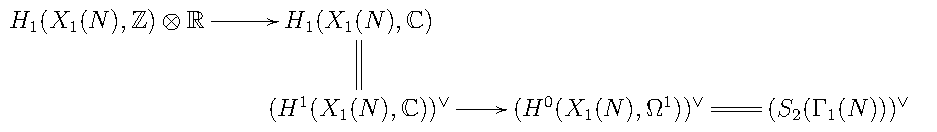
\includegraphics[width=0.7556\paperwidth]{images/L8-p069-homology.pdf}\end{figure}
\end{proposition}
结合\eref{命题}{L8S2O5}与\eref{命题}{L8S3O2}，得到$H_1(X_1(N),\Q)$是$\mathcal H_2(\Gamma_1(N))$上的秩2模。因此，$T_\ell J_1(N)\otimes\Q_\ell$是$\mathcal H_2(\Gamma_1(N))\otimes\Q_\ell$上的秩2自由模。取归一化特征形式$f\in S_2(N,\chi)$，设
\sourcepage{70}
$\lambda$为$\Q(f)$中位于$\ell$上方的素位。存在$\Q$代数同态
\[e_f:\mathcal H_2(\Gamma_1(N))\to\Q(f),\qquad T_n\mapsto a_n(f),\quad\langle d\rangle\mapsto\chi(d).\]
定义
\[V_{f,\lambda}:=(T_\ell J_1(N)\otimes_{\Z_\ell}\Q_\ell)\otimes_{\mathcal H_2(\Gamma_1(N))\otimes\Q_\ell}\Q(f)_\lambda.\]
则$V_{f,\lambda}$是$\Gal(\overline{\Q}/\Q)$在二维$\Q(f)_\lambda$向量空间上的$\ell$进表示，且在$p\nmid\ell N$处非分歧。
\originalnumber{3}
\begin{theorem}\label{L8S3O3}
$\ell$进表示$\sigma_{f,\lambda}:\Gal(\overline{\Q}/\Q)\to\GL(V_{f,\lambda})$与$f$相联系；也就是说，对$p\nmid N\ell$，有
\[\det(1-t\sigma_{f,\lambda}(\mathrm{Fr}_p))=1-a_p(f)t+\chi(p)pt^2.\]
\end{theorem}
若对所有$n\geq1$都有$a_n(f)\in\Z$，则$e_f$将整Hecke代数$\mathcal H_2(\Gamma_1(N))_{\Z}:=\Z[T_n;\langle d\rangle]$满射到$\Z$。因此，存在将$H_1(X_1(N),\Z)$映到$\C$中某个秩2格$\Lambda_f$的映射。由此得到定义在$\Q$上的椭圆曲线$E_f$，并且$\Q(f)=\Q$、$V_{f,\lambda}\cong T_\ell E_f\otimes\Q_\ell$。下面的定理加强了\eref{定理}{L7S2O9}。
\originalnumber{4}
\begin{theorem}{Shimura--Taniyama--Weil猜想}\label{L8S3O4}
每条$\Q$上的椭圆曲线$E$都与某条$E_f$同源，其中$f$是权2、级$N_E$的新形式\znote{「新形式」是相对于「旧形式」而言的：若$f\in S_k(N)$来自更小级数的模形式，即形如$g(mz)$（$m>1$），它就是旧形式；新形式指新子空间（旧形式的正交补）中的归一化特征形式。由重数一性质，归一化特征形式由它的Fourier系数唯一确定，因此「级$N_E$的新形式」与椭圆曲线$E$的对应是唯一确定的。[来源：F. Diamond and J. Shurman, \textit{A First course in Modular forms}, Springer GTM 228 (2005), Chapter 9（本讲参考文献）。]}，$N_E$为$E$的导子。
\end{theorem}
\section{权\texorpdfstring{$k>2$}{k>2}时的主定理}\label{L8S4}
这里只陈述结果，其形式与$k=2$时类似。设$\pi:\mathcal E_Y\to Y_1(N)$为通用族，$j:Y_1(N)\hookrightarrow X_1(N)$为开浸入。
\originalnumber{1}
\begin{proposition}\label{L8S4O1}
存在$\mathcal H_k(\Gamma_1(N))\otimes_{\Q}\R$模的典范同构
% [Tutor Note: 原书 p70 命题 4.1 把 Hecke 代数记作 $T_k(\Gamma_1(N))$，与算子记号 $T_n$ 冲突，应为 $H_k$（即本译本的 $\mathcal H_k$），译文按正确记号处理。]
\[H^1(X_1(N)(\C),j_*\operatorname{Sym}^{k-2}R^1\pi_*\Q)\otimes_{\Q}\R\xrightarrow{\sim}S_k(\Gamma_1(N)).\]
因此，左边的有理上同调空间是$\mathcal H_k(\Gamma_1(N))$上的秩2自由模。
\end{proposition}
取归一化特征形式$f\in S_k(N,\chi)$。对$\Q(f)$中位于$\ell$上方的素位$\lambda$，定义
\[\begin{aligned}
V_{f,\lambda}:={}&H^1_{\mathrm{ét}}(X_1(N)_{\overline{\Q}},j_*\operatorname{Sym}^{k-2}R^1\pi_*\Q_\ell)\\
&\otimes_{\mathcal H_k(\Gamma_1(N))\otimes\Q_\ell}\Q(f)_\lambda.
\end{aligned}\]
\sourcepage{71}
则$V_{f,\lambda}$为$\Gal(\overline{\Q}/\Q)$的二维$\ell$进表示，并在$p\nmid\ell N$处非分歧。
\originalnumber{2}
\begin{theorem}\label{L8S4O2}
$\ell$进表示$\sigma_{f,\lambda}:\Gal(\overline{\Q}/\Q)\to\GL(V_{f,\lambda})$的对偶与$f$相联系；也就是说，对$p\nmid N\ell$，有
\[\det(1-t\sigma_{f,\lambda}^*(\mathrm{Fr}_p))=1-a_p(f)t+\chi(p)p^{k-1}t^2.\]
\end{theorem}
\originalnumber{3}
\begin{note}[L8S4O3]
\eref{定理}{L8S4O2}中取对偶是自然的，因为这里使用的是上同调群；而在$k=2$时，一开始就通过使用同调群而非上同调群取了对偶。
\end{note}
\needspace{5\baselineskip}\section{第8讲参考文献}\label{L8S5}
\needspace{4\baselineskip}\textbf{关于Hecke算子。}
\begin{references}
\refitem{L8bibDS7}{DS} F. Diamond and J. Shurman, \emph{A First course in Modular forms}, Springer GTM 228 (2005), Section 7.9
% [Tutor Note: 原书 p71 此条作者名印作 "J. Churman"，应为 J. Shurman，译文按正确拼写处理。]
\end{references}
\needspace{4\baselineskip}\textbf{关于$Y_1(N)$与$X_1(N)$在$\Z[1/N]$上的约化。}
\begin{references}
\refitem{L8bibDR}{DR} P. Deligne and M. Rapoport, \emph{Les schémas de modules de courbes elliptique}, in W. Kuyk, P. Deligne (eds.) Modular Functions of One Variable II, Lecture Notes in Math., Springer, 349, 1973, 143-316.
% [Tutor Note: 原书 p71 此条作者名印作 "M. Papoport"，应为 M. Rapoport，译文按正确拼写处理。]
\end{references}
\needspace{4\baselineskip}\textbf{关于权$k=2$时Galois表示的构造。}
\begin{references}
\refitem{L8bibDS9}{DS} F. Diamond and J. Shurman, \emph{A First course in Modular forms}, Springer GTM 228 (2005), Chapter 9.
% [Tutor Note: 原书 p71 此条作者名印作 "J. Churman"，应为 J. Shurman，译文按正确拼写处理。]
\refitem{L8bibLW}{LW} D. Loeffler and J. Weinstein, \emph{On the computation of local components of a newform}, In: Math. Comp. 81. 278 (2012), pp. 1179-1200.
\end{references}
\needspace{4\baselineskip}\textbf{关于权$k>2$的情形。}
\begin{references}
\refitem{L8bibD}{D} P. Deligne, \emph{Forms modulaires et représentations $\ell$-adiques}, Séminaire Bourbaki no 355, in Lecture Notes in Math., Springer, 179, 1971, 139-172.
\end{references}
